\section{Introduction}

The software is implemented on an ARM Cortex-M3 supplied by EnergyMicro. This
chapter describes the modules that are executed on this chip.
The responsibility of the software component is mainly producing samples that
the FPGA consumes and to consume the samples the FPGA produces as results.

\begin{figure}[h]
	\centering
	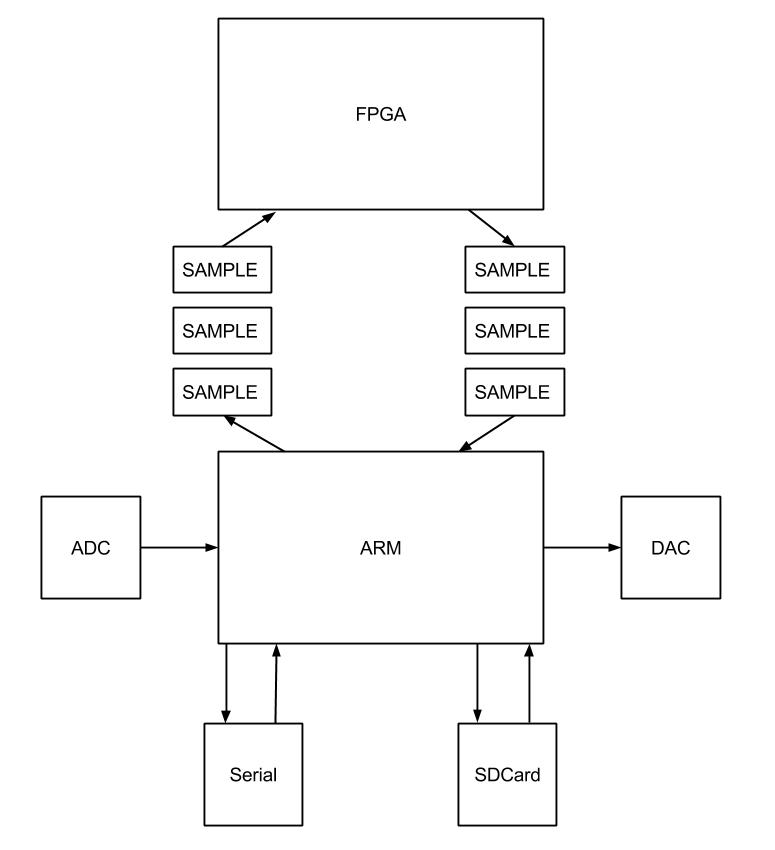
\includegraphics[height=150px]{figures/sw/sample-flow.png}
	%\begin{tikzpicture}[shorten >= 1pt, node distance=3cm, on grid, auto]
	%	\node[draw,rectangle,minimum size=2cm] (fpga) {FPGA};
	%	\node[draw,rectangle,below of=fpga,minimum size=2cm] (arm) {ARM};
	%\end{tikzpicture}
	\caption{Flow of samples}
	\label{fig:sw_sample_flow}
\end{figure}
\todo{Tikzify}


It implements interfaces to the different I/O devices that the system as a whole
uses as source and destination for data samples. These include ADC and DAC
connected to Jack plugs on the card and MicroSD card connected to the SDCard
Slot. In addition a serial port is avaiable for communication with a PC. 

This component also handles general I/O like buttons for controlling the
behavior for of the program at runtime, and leds for visual feedback.

The last responsibility is providing a way to program the FPGA cores. This
functinality is used when the filters used on the FPGA is configured. 
